%%%%%%%%%%%%%%%%%%%%%%%%%%%%%%%%%%%%%%%%%%%%%%%%%%%%%%%%%%%%%%%%%%%%%%%%
%%%  THIS TEX FILE IS TO GENERATE PDF FILE FOR 
%%% 
%%%  COPYRIGHT (C) JIMMY LIN, 2013, UT AUSTIN
%%%%%%%%%%%%%%%%%%%%%%%%%%%%%%%%%%%%%%%%%%%%%%%%%%%%%%%%%%%%%%%%%%%%%%%%
\documentclass[11pt]{beamer}
%%%%%%%%%%%%%%%%%%%%%%%%%%%%%%%%%%%%%%%%%%%%%%%%%%%%%%%%%%%%%%%%%%%%%%%%
%%%  PACKAGES USED IN THIS TEX SOURCE FILE
%%%%%%%%%%%%%%%%%%%%%%%%%%%%%%%%%%%%%%%%%%%%%%%%%%%%%%%%%%%%%%%%%%%%%%%%
\usepackage{graphicx}
\usepackage{wrapfig}
\usepackage{geometry}
\usepackage{color}
\usepackage{JSPPT}
\usepackage[style=ieee]{biblatex}
\usepackage[utf8]{inputenc}
%%%%%%%%%%%%%%%%%%%%%%%%%%%%%%%%%%%%%%%%%%%%%%%%%%%%%%%%%%%%%%%%%%%%%%%%
%%% PRESENTATION INFORMATION
%%%%%%%%%%%%%%%%%%%%%%%%%%%%%%%%%%%%%%%%%%%%%%%%%%%%%%%%%%%%%%%%%%%%%%%%
\title{Multiagent Coordination in Roombas: \newline \ From a Neural Network Perspective}
\author[Jimmy Lin and Barry Feigenbaum]{\bf Jimmy Lin \\Barry Feigenbaum}
\institute{\bf Prof. Risto Miikkulainen\\[0.3cm] Department of Computer Science \\The University of Texas At Austin}

%%%%%%%%%%%%%%%%%%%%%%%%%%%%%%%%%%%%%%%%%%%%%%%%%%%%%%%%%%%%%%%%%%%%%%%%
%%% TITLE PAGE
%%%%%%%%%%%%%%%%%%%%%%%%%%%%%%%%%%%%%%%%%%%%%%%%%%%%%%%%%%%%%%%%%%%%%%%%
\AtBeginSection{\frame{\sectionpage}}
\setbeamertemplate{itemize item}[ball]
\setbeamertemplate{itemize subitem}{--}

\begin{document}
\begin{large}
    \frame{\maketitle}%\titlepage
\end{large}

\frame{
    \frametitle{Table of Contents}
    \tableofcontents
}

%%%%%%%%%%%%%%%%%%%%%%%%%%%%%%%%%%%%%%%%%%%%%%%%%%%%%%%%%%%%%%%%%%%%%%%%
%%% DOCUMENTATION STARTS FROM HERE
%%%%%%%%%%%%%%%%%%%%%%%%%%%%%%%%%%%%%%%%%%%%%%%%%%%%%%%%%%%%%%%%%%%%%%%%

\section{Problem Motivation}
% recapture contents of previous topic talks
\frame{
    \frametitle{Structure of the Roomba Environment}

    \begin{itemize}
        \item Objects: 

    \begin{itemize}
        \item Agent: dynamic dirt collectors (Black Disks)
        \item Scrumb: static dirt to clean (Blue Dots)
        \item Wall: static boundary of the world 
    \item Chair/Desk: static decorations as hidden obstacles
    \end{itemize}

    Roomba pictures
\item Objectives: 
    \begin{itemize}
        \item collect as many scrumbs as possible
        \item make as few collision as possible
    \end{itemize}
    \end{itemize}
}

\frame{
    \frametitle{A Ideal Case}
    \begin{itemize}
        \item The most ideal case is to set up a system with 

    \begin{itemize}
        \item  Centrailization: full control over all agents 
        \item  Global View: full observations over all scrumbs 
    \end{itemize}
    
\item In this system, the crumb collection can be formulated as 
    an integer programming problem. 
\item No experiential learning is needed in this case.

\end{itemize}
}

\frame{
    \frametitle{A Slightly Realisitc Case}
    \begin{itemize}
        \item Relax the "Centralization" assumption and yield a decentralized system
    with
    \begin{itemize}
        \item  Autonomy: all agents should decide on its own
        \item  Global View: full observations over all scrumbs are still available
            for all agents
    \end{itemize}
    \item  We need 
    \begin{itemize}
        \item Local policy optimizers that approximates the globally optimal policies
        \item Collision-free or collision-tolerant protocol between agents
    \end{itemize}
    \end{itemize}
}

\frame{
    \frametitle{A More Realisitc Case}
    \begin{itemize}
        \item Relax the "Global View" assumption, but allow limited information sharing
    between agents. These yield a system with
    \begin{itemize}
        \item  Autonomy: all agents should decide on its own
        \item  Local View: only local observation of scrumbs are available for
            agents
        \item  Limited Sharing: a small amount of information is shared between agents
    \end{itemize}
\item We are going to solve the maximum crumbs collection problem using
    experiential learning.
    \end{itemize}
    
}

%%%%%%%%%%%%%%%%%%%%%%%%%%%%%%%%%%%%%%%%%%%%%%%%%%%%%%%%%%%%%%%%%%%%%%%%
\section{Approaches and Architectures}
\frame{
    \frametitle{Challenges and Difficulties}

    \begin{itemize}
        \item Communication:  
    \begin{itemize}
        \item  what information to share?
        \item  how to share it for the best performance?
    \end{itemize}
        \item Learning Mechanism: What learning policy makes the learning simplest and fastest? 
    \begin{itemize}
        \item Enforced SubPopulation (ESP).
        \item Opportunistic Cooperative Learning (OCL).
    \end{itemize}
        \item Sensors: 
    \end{itemize}
}

\frame{
    \frametitle{Approaches}
    \begin{itemize}
    \item Learning mechanisms:
    	\begin{itemize}
    	\item Neroevolution (Real-time NEAT)
    	\item Q-learning
    	\end{itemize}
    \item Techniques to support cooperation:
    	\begin{itemize}
        \item Communication between agents
        \item Social learning
        \item Centralized control / coordination
        \end{itemize}
    \item Compare against hardcoded behavior as a baseline:
    	\begin{itemize}
    	\item Random agents
    	\item Purely greedy search
    	\end{itemize}
    \end{itemize}
}


%%%%%%%%%%%%%%%%%%%%%%%%%%%%%%%%%%%%%%%%%%%%%%%%%%%%%%%%%%%%%%%%%%%%%%%%
\section{Experimental Results}

\frame{
    \frametitle{Results}
	\begin{itemize}
	\item Initial results are unexciting - agents don't learn
	\item Roomba module needs considerable work just to be used as a baseline
	\item Most of our effort has been spent getting the Roomba mod on track
	\item A major issue is learning obstacle avoidance
	\end{itemize}
}

\frame{
    \frametitle{Unmodified Roomba Environment}
	\begin{center}
	    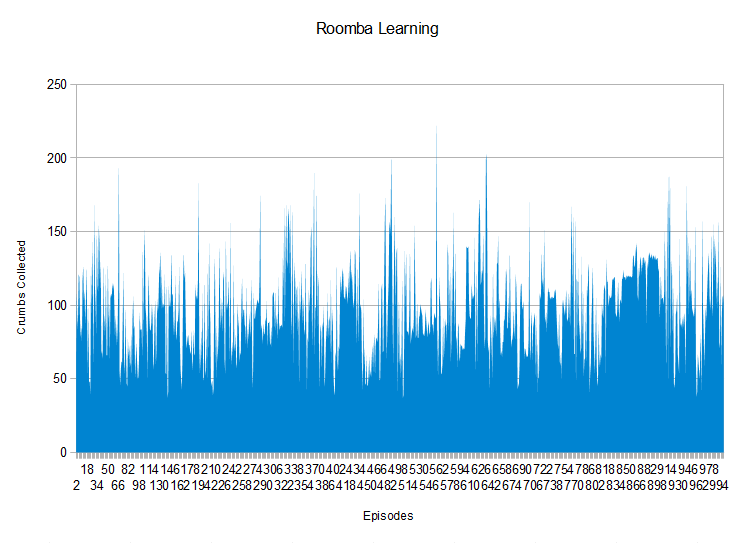
\includegraphics[height=7cm]{figs/roomba_learning_1000gen.png}
	\end{center}
}

\frame{
    \frametitle{Conclusions}
	\begin{itemize}
	\item 
	\end{itemize}
}

%\frame{
%    \frametitle{Future Work}
%}

\section{Discussion}
\frame{
    \frametitle{Discussion Time}
    \begin{itemize}
        \item Any questions or suggestions?  \\
            [insert pictures]
        \item Or email us at 
            \begin{itemize}
                \item jimmylin at utexas dot edu
                \item chevron8 at gmail dot com
            \end{itemize}
    \end{itemize}
}

%%%%%%%%%%%%%%%%%%%%%%%%%%%%%%%%%%%%%%%%%%%%%%%%%%%%%%%%%%%%%%%%%%%%%%%%
%%% REFERENCES
%%%%%%%%%%%%%%%%%%%%%%%%%%%%%%%%%%%%%%%%%%%%%%%%%%%%%%%%%%%%%%%%%%%%%%%%
%\appendix
%\section{Appendix}
%\frame[allowframebreaks]{
%    \frametitle{References}
%    \begin{thebibliography}{9}
%    	\bibitem{bryant03} Bobby D. Bryant and Risto Miikkulainen (2003). Neuroevolution for Adaptive Teams. {\it Proceedings of the 2003 Congress on Evolutionary Computation} 1:2194-2201. 
%    
%        \bibitem{tan1993multi} Tan, Ming. "Multi-agent reinforcement learning:
%        Independent vs. cooperative agents." {\it Proceedings of the Tenth
%            International Conference on Machine Learning}. Vol. 337. 1993.
%        
%        \bibitem{rawar} Rawal, A.; Rajagopalan, P.; Miikkulainen, R., "Constructing competitive and cooperative agent behavior using coevolution," {\it Computational Intelligence and Games (CIG), 2010 IEEE Symposium on}, vol., no., pp.107,114, 18-21 Aug. 2010
%        
%        \bibitem{rajagopalan11} Rajagopalan, P.; Rawal, A.; Miikkulainen, R.; Wiseman, M.A.; Holekamp, K.E., "The role of reward structure, coordination mechanism and net return in the evolution of cooperation," {\it Computational Intelligence and Games (CIG), 2011 IEEE Conference on}, vol., no., pp.258,265, Aug. 31 2011-Sept. 3 2011
%        
%    	\bibitem{risto12} Risto Miikkulainen and Eliana Feasley and Leif Johnson and Igor Karpov and Padmini Rajagopalan and Aditya Rawal and Wesley Tansey (2012). {\it Multiagent Learning through Neuroevolution. Advances in Computational Intelligence} LNCS 7311:24-46.     
%        
%        \bibitem{yang02} Yanli Yang; Polycarpou, M.M.; Minai, A.A., "Opportunistically cooperative neural learning in mobile agents," {\it Neural Networks, 2002. IJCNN '02. Proceedings of the 2002 International Joint Conference on}, vol.3, no., pp.2638,2643, 2002
%        
%        \bibitem{yong09} Yong, C.H.; Miikkulainen, R., "Coevolution of Role-Based Cooperation in Multiagent Systems," {\it Autonomous Mental Development, IEEE Transactions on}, vol.1, no.3, pp.170,186, Oct. 2009
%    \end{thebibliography}
%}

\frame{
    \frametitle{Acknowledgement}
    Thanks.
}
\end{document}
